\documentclass{article}

\usepackage[final]{nips_2018}

% to avoid loading the natbib package, add option nonatbib:
% \usepackage[nonatbib]{nips_2018}

\usepackage[utf8]{inputenc} % allow utf-8 input
\usepackage[T1]{fontenc}    % use 8-bit T1 fonts
\usepackage{hyperref}       % hyperlinks
\usepackage{url}            % simple URL typesetting
\usepackage{booktabs}       % professional-quality tables
\usepackage{amsfonts}       % blackboard math symbols
\usepackage{nicefrac}       % compact symbols for 1/2, etc.
\usepackage{microtype}      % microtypography

\usepackage{graphicx}
\usepackage{cite}

\title{BLACK: Body Language Affect Classification Kernel}

\author{
  Undergrad-ient Descent Expedition: \\
  Jack (Xiang) Zhou, Karan Aujla, James Bie, Eric Gao, Insoo Rhee\\
  Faculty of Applied Sciences\\
  Simon Fraser University\\
  Burnaby, Canada\\
  \texttt{xza194@sfu.ca} \\
}

\begin{document}

\maketitle

\begin{abstract}
  This is the abstract of the paper that we are going to write
\end{abstract}

\section{Introduction}



Task is to assign affective label on humans, face based affective label assignment is not very good atm, use body as a supplement.

Task is difficult even for humans. 

Talk about COBOL \citep{schindler2008recognizing}, work has been done before with a neurologically inspired model but not on a skeleton level

Happy is most compact and separable from other emotions in multiple findings, link that back to our own findings later on.

\section{Approach}
\subsection{Architecture}

We introduce the general architecture of the overall pipeline in this section. The novel and primary goal of the present work is to assign affective labels with learned patterns in body langauge. However, as we are only in the primary stage in this pursuit and we do not have a comprehensive method toward accounting for viewpoint invariance, using body posture as the primary is not very realistic. In the present work we use body language mainly as a supplement to existing facial affective labels if it is detected.

A snapshot is taken from an arbitrary visual stream and the resulting image is passed into OpenPose to detect all persons. For each person: (1) If a face was found, then it is passed into a face-based classifier for an evaluation of the affective rating vector based solely on face. (2) If a body was found, then it is passed into a body language-based classifier for an evaluation of the affective rating vector based solely on body. A weighted sum is computed between (1) and (2) for each person. If only one of (1) or (2) is found, then only that one is taken. A grand total is calculated by summing over every person's weighted sum of affective labels. The grand total will be passed into a softmax function to obtain a probability vector of the model prediction. A graphical depiction of this overall process is shown in Figure 1.

\begin{figure}[h]
	\centering
	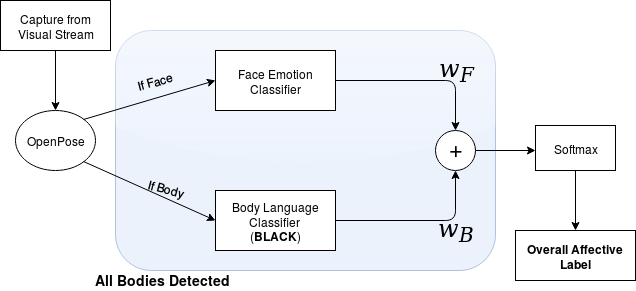
\includegraphics[scale=0.5]{Pipeline}
	\caption{The overall pipeline.}
\end{figure}

\subsubsection{Body Language Keypoint Estimation}

To extract body keypoints, we used the OpenPose system produced by the CMU Perceptual Computing Laboratory \citep{cao2017realtime} \citep{simon2017hand} \citep{wei2016cpm}

Openpose is a system the detects people in an image or video and finds the estimated location of several keypoints on their body, hands, and face. It is a capable of finding the keypoints of multiple people in the same image. Openposes’s	 basic algorithm finds each type of keypoint in all bodies at the same time and finds the connection between keypoints in a separate neural network. This program can take most image and video formats as inputs, such as jpeg, png, avi, and mp4 formats. It will output in a variety of formats depending on the flags given. For example, it can output an image with the skeletons overlaid on the people in the image, and output json files for the keypoints. In the json file, it contains the x, y coordinates of every bone detected, as well as a confidence rating for the position of each bone. Openpose can output the json in a variety of formats, such as grouping each x,y,c tuple into it’s own object. For our model, openpose is configured to output a json file containing a separate object for each bone and to normalize the coordinates to [-1,1]. Then we find the angles of each bone to ensure that the input values are position invarient

\subsubsection{Face Emotion Classification}
aaaaaaa
\subsection{Training}
As the problem that the present model is trying to solve involve uncensored face along with body posture, it is particularly difficult to obtain relevant published datasets that are labelled and publicly available. Past research in this field involved manual construction of data from actors \citep{schindler2008recognizing}.

To address this issue, we manually construct a dataset of unlabelled images of humans with visible face and body posture by using authors of this paper as actors as well as sources on the internet. The face and body are both clearly visible in the training images. The image will not be given a label when it is fed into the training pipeline in a pseudounsupervised learning paradigm. We describe the training pipeline as follows:

\begin{figure}[h]
	\centering
	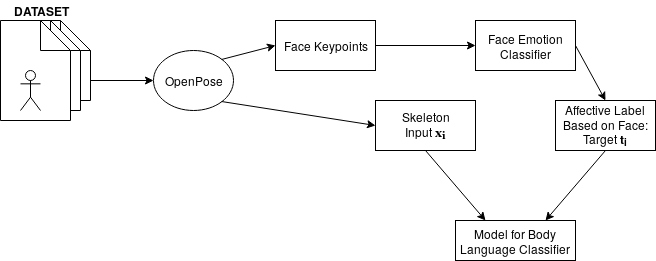
\includegraphics[scale=0.6]{tpipeline}
	\caption{The training pipeline.}
\end{figure}

The unlabelled image is first passed into OpenPose to obtain a set of posture keypoints (ie. a skeleton) of the human in the image, as well as a set of face keypoints. The face keypoints will be passed into an already trained face emotional classifier to give a ground truth affective label for the overall human in the image as informed by the face. The skeleton is then processed into an invariant form and used along with the affective label to train the body language affect classifier.

\section{Experiments}

\section{Conclusion}

\subsection{Future Work}

using a generalized linear model to deal with multiple persons instead of a simple sum

fitting LSTM to generalize into videos

accounting for Confidence in body keypoint measurements dynamically

\section{Contributions}

As with most group projects, each author of this paper contributed a considerable amount of work towards piecing together the project. Jack oversaw the project by organizing and delegating tasks for everyone as well as being the main composer of the paper and poster. Jack and James formulated the design of the overall pipeline for the models and for training the model. Karan worked with existing models for body posture keypoint extraction and implemented the top level program. Eric and James are the main contributors to data collection and piecing together a custom dataset for the project. Insoo and Jack worked on designing and implementing the model for mapping body keypoints to affective labels.

We would also like to thank Professor Angelica Lim for consultations and guidance toward the design and theoretical groundwork for the project.

\bibliography{references.bib}
\bibliographystyle{plain}

\end{document}
